\chapter{Complessità computazionale e calcolo quantistico}
\label{ch:qc}
In questo capitolo introduciamo i concetti di base del calcolo quantistico. Esaminiamo le ragioni che ci spingono a cercare nuovi paradigmi computazionali e perché il calcolo quantistico appare promettente.

Per comprendere appieno le aspettative riposte nel calcolo quantistico, è necessario innanzitutto introdurre alcuni elementi di calcolabilità e complessità. Esamineremo quindi i fondamenti dell'informatica a partire dai modelli computazionali. Daremo una definizione di problema computazionale e vedremo quali problemi possiamo risolvere con un computer. Infine, studieremo la complessità computazionale dei problemi classificandoli in base alle risorse necessarie per trovare una soluzione.

Completata questa introduzione allo studio della complessità computazionale, vedremo come i computer quantistici si inseriscono in questa analisi. Inizieremo presentando un modello computazionale che ci permette di definire quali problemi sono risolvibili su un computer quantistico, e osserveremo come questo ci porti naturalmente verso i computer quantistici basati su porte quantistiche. Vedremo quali classi di complessità possono essere definite considerando questo nuovo paradigma, e cercheremo di comprendere quali relazioni esistono tra le classi di problemi identificate con il modello classico di computazione e quelle derivate dal modello quantistico.

Nella seconda sezione di questo capitolo presenteremo in modo più rigoroso i computer basati su porte quantistiche. Vedremo cosa si intende per porta quantistica, presenteremo le porte più comuni e costruiremo un insieme universale di porte. Vedremo poi cosa significa programmare un computer basato su porte quantistiche presentando l'algoritmo di Deutsch.

Il capitolo si conclude presentando l'\emph{Adiabatic Quantm Computing} (AQC) (Computazione Quantistica Adiabatica): un paradigma alternativo alla computazione basata su porte quantistiche. Descriveremo i fondamenti teorici di questo paradigma e mostreremo che l'AQC e il calcolo basato su porte quantistiche sono equivalenti. Vedremo che programmare una macchina che sfrutta il paradigma AQC significa tradurre il problema che vogliamo risolvere in un problema di minimizzazione.
Presentiamo un altro approccio nativamente implementabile con l'AQC: il \emph{Quantum Annealing} QA. Descriveremo il QA tracciando un parallelo tra il simulated annealing classico e il quantum annealing. Infine, ci concentreremo sulla formulazione di problemi di minimizzazione naturalmente risolvibili con il quantum annealing.

Questo capitolo è ispirato ai seguenti libri e articoli: la Sezione~\ref{sec:complexity} è ispirata a \cite[capitoli $3$ e $4$]{nielsen2010quantum}, la Sezione~\ref{sec:gate_model} è tratta da \cite[capitoli $2$, $3$, $4$ e $7$]{nielsen2010quantum}, infine la Sezione~\ref{sec:qac_model} è ispirata a \cite[capitoli $2$ e $3$]{mcgeoch2022adiabatic} e \cite{k2005transverse}. Nelle pagine seguenti questi riferimenti non vengono più considerati e, quando necessario, citiamo altri lavori.

\section{Introduzione all'analisi computazionale}
L'analisi della complessità computazionale si occupa di studiare quali problemi possono essere risolti tramite un computer e quali risorse sono necessarie per trovare la soluzione. Possiamo dividere questi due obiettivi in due linee di ricerca parallele e complementari. Da un lato, per dimostrare che un problema è risolvibile, è sufficiente mostrare un algoritmo capace di risolverlo, senza preoccuparsi troppo della sua complessità. Dall'altro, per capire quali risorse sono necessarie, vorremmo trovare un limite inferiore alle operazioni che devono essere eseguite per ottenere la soluzione.

Queste linee di ricerca sono complementari nel senso che, idealmente, una volta identificato un limite inferiore, vorremmo essere in grado di costruire un algoritmo che lo raggiunga. In pratica, questo non è sempre possibile, perché costruire algoritmi che si comportino bene su tutte le istanze di un problema è difficile, e perché il limite inferiore delle operazioni richieste non è sempre noto, quindi ci si deve accontentare del miglior algoritmo sviluppato finora.

Abbiamo fatto riferimento a un algoritmo sapendo intuitivamente che è una sequenza di operazioni che ci permette di trovare la risposta a un problema. Per studiare formalmente le caratteristiche di un algoritmo, questa intuizione non è sufficiente; abbiamo bisogno di qualcosa che possiamo caratterizzare in modo più preciso. Introduciamo quindi i modelli computazionali.
\subsection{Modelli computazionali}
\label{sec:complexity}
Un modello computazionale ci permette di definire matematicamente il concetto di algoritmo. Queste astrazioni furono introdotte per la prima volta da Turing e Church per trovare una soluzione all'\emph{entscheidungsproblem} di Hilbert\footnote{Per ogni problema matematico, esiste un algoritmo capace di risolverlo?}. Consideriamo ora due modelli computazionali equivalenti: la \emph{macchina di Turing} e il \emph{modello a circuiti}. 
\subsubsection*{Macchina di Turing}
Questo è il modello computazionale più noto. Introdotto da Turing per descrivere formalmente la nozione di algoritmo che esegue un compito computazionale.

Una \marginpar{Definizione di\\macchina di Turing}macchina di Turing può essere vista come la concettualizzazione di un computer. È composta da quattro elementi principali:
\begin{description}
	\item[Programma:] che consente la codifica di un algoritmo;
	\item[Controllo a stati finiti:] unità che funge da processore;
	\item[Nastro:] memoria del computer;
	\item[Testina di lettura-scrittura:] interagisce con la memoria.
\end{description} 

È possibile definire varie versioni della macchina di Turing. Per la nostra discussione possiamo considerare la versione più semplice, in cui il nastro di memoria è illimitato a destra e limitato a sinistra. I simboli che possono essere scritti sul nastro sono $0$, $1$, $b$ (il simbolo vuoto) e il simbolo speciale $\triangleright$ che segna l'estremità sinistra del nastro. Questi simboli formano il nostro alfabeto $\Gamma$: tutto ciò che può essere rappresentato sul nastro consiste in stringhe di lunghezza finita $\Gamma^*$ composte da simboli dell'alfabeto (tranne $\triangleright$, che appare solo all'inizio del nastro). Il controllo a stati finiti consiste in un insieme finito di stati $q_1, \dots, q_m$ più due stati speciali $q_s$ e $q_h$ che rappresentano, rispettivamente, lo stato iniziale della macchina e lo stato finale (di arresto); quest'ultimo viene raggiunto quando la macchina ha terminato il calcolo. 

Un programma per la macchina di Turing consiste in righe di programma; ogni riga è una quintupla $\braket{q, x, q', x', s}$ che viene interpretata come segue: se la macchina si trova nello stato $q$ e legge il simbolo $x \in \Gamma$ sul nastro, allora transita nello stato $q'$, scrive il simbolo $x' \in \Gamma$ sul nastro e si muove come indicato da $s$ (a destra $+1$, a sinistra $-1$, oppure rimane ferma $0$).

Il modello della macchina di Turing può sembrare semplice, ma è il formalismo di riferimento per stabilire cosa consideriamo calcolabile o meno. L'importanza della macchina di Turing è supportata dalla \emph{tesi di Church–Turing} proposta indipendentemente da Church e Turing:
\begin{thesis}\marginpar{\\Tesi di Church–Turing}
	La classe delle funzioni calcolabili da una macchina di Turing corrisponde esattamente alla classe delle funzioni che naturalmente considereremmo calcolabili da un algoritmo.
\end{thesis}
La tesi di Church–Turing afferma che la macchina di Turing è un modello computazionale capace di fornire una definizione rigorosa del concetto intuitivo di algoritmo, ed è quindi adatta come fondamento dell'informatica.

La macchina di Turing che abbiamo descritto può essere modificata, ad esempio immaginando di avere più nastri di memoria; questa nuova macchina potrebbe essere in grado di risolvere i problemi più rapidamente dell'originale, ma saremo sempre in grado di simulare la macchina multinastro con una macchina a nastro singolo. Ciò significa che considerare nastri multipli non aumenta la potenza della macchina di Turing.

Un'altra modifica, che sarà utile in seguito, che possiamo apportare a questo modello computazionale è considerare una versione probabilistica della macchina di Turing: se la macchina si trova nello stato $q$ e il simbolo $x$ viene letto, si lancia una moneta; se il risultato è testa, la macchina transita nello stato $q_H$, altrimenti nello stato $q_T$. Anche questa modifica può essere simulata con una macchina di Turing che esplora tutti i possibili percorsi di calcolo uno alla volta (usando un numero esponenzialmente maggiore di passi), quindi ancora una volta l'insieme delle funzioni calcolabili non viene esteso.

\paragraph{Indecidibilità:} I modelli computazionali, e con essi l'informatica, furono sviluppati per rispondere all'entscheidungsproblem di Hilbert. Church, con il $\lambda$-calcolo\footnote{Un altro modello computazionale equivalente alla macchina di Turing.}, e Turing, con la macchina di Turing, dimostrarono che la risposta è no: non può esistere un algoritmo per decidere tutti i problemi della matematica.

Questo risultato divide chiaramente i problemi matematici in due classi: quelli che possono essere risolti con un algoritmo e quelli così difficili da essere computazionalmente irrisolvibili. Chiamiamo i problemi appartenenti a questa classe \emph{indecidibili}. Turing dimostra che il \emph{problema della fermata} (il problema di determinare se una macchina di Turing si ferma dato un input) è, in generale, indecidibile\footnote{Church dimostra che non esiste una funzione calcolabile che permetta di determinare se due espressioni del $\lambda$-calcolo sono equivalenti.}. Oltre ai problemi usati nelle dimostrazioni di Church e Turing, esistono molti altri problemi indecidibili, ad esempio trovare un omeomorfismo tra due spazi topologici o alcuni problemi relativi al comportamento dei sistemi dinamici. 

\subsubsection*{Modello a circuiti}
Il modello a circuiti è un modello alternativo di computazione in cui descriviamo un algoritmo implementandolo tramite un circuito composto da porte logiche. Questo approccio è interessante perché ci avvicina al primo modello quantistico di computazione: il modello basato su porte.

\begin{figure}[H]
	\centering
	\begin{subfigure}[c]{.21\linewidth}
		
\includegraphics[width=.95\linewidth]{quantum_computing/not}
		\caption{Porta \smallcaps{not}}
		\label{fig:not}
	\end{subfigure}
	\hfill
	\begin{subfigure}[c]{.21\linewidth}
		
\includegraphics[width=.95\linewidth]{quantum_computing/and}
		\caption{Porta \smallcaps{and}}
		\label{fig:end}
	\end{subfigure}
	\hfill
	\begin{subfigure}[c]{.21\linewidth}
		
\includegraphics[width=.95\linewidth]{quantum_computing/or}
		\caption{Porta \smallcaps{or}}
		\label{fig:or}
	\end{subfigure}
	\hfill
	\begin{subfigure}[c]{.21\linewidth}
		
\includegraphics[width=.95\linewidth]{quantum_computing/xor}
		\caption{Porta \smallcaps{xor}}
		\label{fig:xor}
	\end{subfigure}
	\caption{Porte logiche}
	\label{fig:gate}
\end{figure}

Nella Figura~\ref{fig:gate} sono mostrate le porte logiche più note, con le quali possiamo costruire un circuito digitale. A queste aggiungiamo normalmente la possibilità di ottenere una copia di un bit (un filo che si divide), un'operazione che chiamiamo \smallcaps{fanout}, e la possibilità di scambiare due bit, chiamata \smallcaps{crossover}.

È possibile dimostrare che con questo insieme limitato di porte si può calcolare qualsiasi funzione $f : \Set{0,1}^n \rightarrow \Set{0,1}^m$. Questo non è sufficiente per descrivere un modello computazionale utile. Prima di vedere quali caratteristiche richiediamo, definiamo il concetto di famiglia di circuiti.

Una \emph{famiglia di circuiti} è un insieme di circuiti $\Set{C_n}$ indicizzati da $n\in\mathbb{N}$. Il circuito $C_n$ ha $n$ bit di input e un numero finito di bit di lavoro extra e bit di output. Dato un circuito $C_n$ e una stringa di bit $x$ di lunghezza massima $n$ come input del circuito, denotiamo con $C_n(x)$ l'output del circuito. 

Diciamo che una famiglia di circuiti è \emph{consistente} se tutti i circuiti nella famiglia calcolano la stessa funzione $C(\cdot)$. Formalmente, la definizione di consistenza è: la famiglia di circuiti $\Set{C_n}$ è consistente se per $m < n$ e $x$ di lunghezza al più $m$ bit, allora $C_m(x) = C_n(x)$. 

Infine, definiamo una famiglia di circuiti \emph{uniforme} se esiste un algoritmo per una macchina di Turing che, dato $n$ come input, è in grado di generare una descrizione di $C_n$. Cioè, questo algoritmo deve fornire l'elenco delle porte che costituiscono $C_n$, e la descrizione di come queste porte sono collegate tra loro.

Siamo \marginpar{Definizione del\\modello a circuiti}finalmente pronti a descrivere le caratteristiche formali del modello computazionale a circuiti. In questo modello consideriamo le funzioni calcolabili da famiglie di circuiti $\Set{C_n}$ tali che:
\begin{itemize}
	\item i circuiti nella famiglia sono \emph{aciclici}: nel circuito non devono essere presenti cicli, questo previene il verificarsi di possibili instabilità;
	\item $\Set{C_n}$ è una famiglia di circuiti \emph{consistente}: tutti i circuiti calcolano la stessa funzione (su input di dimensione crescente);
	\item $\Set{C_n}$ è una famiglia di circuiti \emph{uniforme}: i circuiti possono essere generati a partire da un algoritmo ragionevole. 
\end{itemize}

È possibile dimostrare che la classe di funzioni calcolabili da una famiglia di circuiti consistente, uniforme e aciclica è esattamente la stessa calcolabile su una macchina di Turing.

\subsection{Problemi computazionali}
I modelli teorici che abbiamo definito nella sezione precedente (e altri equivalenti che sono stati proposti nel corso dello studio dell'informatica) ci permettono di studiare formalmente i problemi computazionali. Questa analisi dipende dalla risposta a tre domande fondamentali:
\begin{description}
	\item[Cos'è un problema computazionale:] i problemi computazionali sono una classe specifica di problemi chiamati \emph{problemi decisionali}. Questa scelta ci permette di isolare una classe ristretta per semplificare l'analisi e fare progressi nello sviluppo della teoria. Vedremo che i risultati ottenuti si estendono ben oltre i problemi decisionali;
	\item[Come sviluppare un algoritmo per risolverlo:] dopo l'identificazione del problema, è necessario sviluppare un algoritmo capace di trovare una soluzione. Siamo poi interessati a determinare se esistono algoritmi generali capaci di risolvere ampie classi di problemi. Infine, vorremmo trovare strumenti per garantire che un algoritmo funzioni effettivamente come previsto;
	\item[Quali risorse sono necessarie per la soluzione:] un algoritmo consuma risorse computazionali come tempo, spazio ed energia; vogliamo sapere se l'algoritmo sviluppato consuma più risorse di quelle effettivamente necessarie. Inoltre, vorremmo classificare i problemi in base alle risorse richieste per risolverli.
\end{description}

\subsubsection*{Complessità computazionale}
Lo studio della complessità computazionale mira a quantificare le risorse computazionali necessarie per risolvere un dato problema. Per \marginpar{Notazione asintotica}studiare il consumo di risorse indipendentemente dalle caratteristiche dell'architettura di riferimento\footnote{Intendiamo l'indipendenza da specifiche scelte architetturali che, ad esempio, consentono a un processore di risparmiare qualche ciclo di clock ogni volta che viene eseguita una certa operazione. Vedremo presto che diversi modelli computazionali possono, invece, avere un consumo di risorse asintoticamente diverso.}, viene introdotta la \emph{notazione asintotica}, che cattura il comportamento essenziale di una funzione:
\begin{itemize}
	\item $O$ (\say{O grande}): usato per definire il \emph{limite superiore} di una funzione;
	\item $\Omega$ (\say{Omega grande}): usato per definire il \emph{limite inferiore} di una funzione;
	\item $\Theta$ (\say{Theta grande}): è la combinazione di $O$ e $\Omega$, descrive il comportamento asintotico di una funzione.
\end{itemize}

La complessità computazionale considera le risorse spaziali e temporali necessarie per risolvere un problema e cerca di dimostrare l'esistenza di un limite inferiore per queste risorse indipendentemente dall'esistenza o meno di un algoritmo ottimale che rispetti questo limite inferiore. Chiaramente, lo sviluppo di algoritmi dovrebbe mirare a trovare un algoritmo che non utilizzi più risorse del necessario, ovvero il limite inferiore teorico identificato dallo studio della complessità computazionale.

Nello sviluppo della teoria della complessità computazionale, si è osservato che il consumo di risorse dipende dal modello computazionale di riferimento; ad esempio, le tre diverse macchine di Turing presentate nella sezione precedente possono risolvere lo stesso problema con un numero di operazioni molto diverso.

Questo \marginpar{Problemi facili e difficili} problema è stato chiaramente affrontato dividendo i problemi in due classi:
\begin{itemize}
	\item problemi \emph{facili}, \emph{trattabili} o \emph{gestibili}: sono problemi per i quali esiste un algoritmo capace di trovare una soluzione in tempo \emph{polinomiale} rispetto alla dimensione del problema. Un algoritmo il cui consumo di risorse cresce come $O(p(n))$, dove $n$ è la dimensione del problema e $p(\cdot)$ è un polinomio, è chiamato \emph{efficiente};
	\item problemi \emph{difficili}, \emph{intrattabili} o \emph{ingestibili}: se il miglior algoritmo richiede risorse esponenziali\footnote{Consideriamo esponenziale tutto ciò che cresce più velocemente di un polinomio; $n^{\log n}$, con un certo abuso di notazione, è considerata una funzione esponenziale.}. In questo caso si parla di algoritmi \emph{inefficienti}.
\end{itemize}

Ci sono diverse ragioni per cui la scelta di dividere i problemi in due classi di complessità computazionale (polinomiale ed esponenziale) è appropriata. La prima è storica: i polinomi che descrivono la maggior parte degli algoritmi proposti non hanno grado elevato, il che significa che gli algoritmi polinomiali quasi sempre superano quelli esponenziali. La seconda ragione è più fondazionale ed è dovuta alla \emph{tesi forte di Church–Turing}:
\begin{thesis}\marginpar{\\Tesi forte di\\Church–Turing}
	Qualsiasi modello di computazione può essere simulato su una macchina di Turing probabilistica con al più un aumento polinomiale nel numero di operazioni elementari richieste.
\end{thesis}
Ciò significa che le macchine di Turing probabilistiche sembrano essere il modello di computazione \say{ragionevole} più potente. Formalmente, possiamo affermare che se, considerando un certo modello computazionale (diverso dalla macchina di Turing probabilistica), è possibile risolvere un problema con $k$ operazioni elementari, allora è possibile risolvere lo stesso problema su una macchina di Turing probabilistica con al più $p(k)$ operazioni elementari (dove $p(\cdot)$ è un polinomio).

Invertendo questa descrizione, la tesi forte di Church–Turing afferma che, dato un certo problema da risolvere, se non esiste un algoritmo efficiente per la macchina di Turing probabilistica, allora non esiste un algoritmo efficiente per nessun dispositivo computazionale.

\subsubsection*{Classi di problemi}
Finora abbiamo diviso i problemi in polinomiali ed esponenziali; consideriamo ora suddivisioni più fini dei problemi computazionali, tenendo conto non solo del tempo richiesto ma anche dello spazio necessario per trovare la soluzione. Prima di dividere i problemi in classi, definiamo formalmente i problemi decisionali introdotti all'inizio di questa sezione.

Un problema decisionale è un problema la cui risposta è sì o no. Possiamo definirli formalmente usando la terminologia dei \emph{linguaggi formali}. Un linguaggio $L$ sull'alfabeto $\Gamma$ è un sottoinsieme dell'insieme $\Gamma^*$ di tutte le stringhe (finite) di simboli di $\Gamma$. Una stringa rappresenta l'input del nostro problema e può essere scritta sul nastro di una macchina di Turing. La macchina esegue un calcolo che può terminare scrivendo sul nastro una stringa equivalente a sì o no a seconda che la stringa di input appartenga al linguaggio $L$ o meno.

In generale, un linguaggio $L$ è \emph{deciso} da una macchina di Turing se la macchina è in grado di decidere se un input $x$ sul suo nastro è un elemento del linguaggio $L$ oppure no.

\paragraph{Classe P:} Diciamo che un problema può essere risolto in tempo polinomiale se esiste una macchina di Turing capace di decidere se l'input $x$ di dimensione $n$ appartiene al linguaggio in tempo $O(n^k)$ per qualche $k$ finito; diciamo che questo problema appartiene a \textbf{TIME}$(n^k)$. L'insieme di tutti i linguaggi in \textbf{TIME}$(n^k)$ è denotato con \textbf{P}. \textbf{P} è il nostro primo esempio di \emph{classe di complessità}.

Per dimostrare che un linguaggio $L$ appartiene a \textbf{P}, è sufficiente mostrare un algoritmo che decide $L$ in tempo polinomiale. Purtroppo, esistono problemi per i quali tale algoritmo non è stato ancora trovato. Ci si può quindi chiedere se esistano problemi al di fuori di \textbf{P}.

Viceversa, sebbene esistano dimostrazioni non costruttive che mostrano che devono esistere problemi che richiedono risorse esponenziali, sembra molto difficile dimostrare che un problema specifico non appartiene a \textbf{P}.

\paragraph{Classe NP:} Esistono problemi per i quali non è stato trovato un algoritmo polinomiale, ma se la soluzione al problema viene in qualche modo fornita, è possibile applicare un algoritmo efficiente per verificare tale soluzione. I problemi con questa proprietà appartengono alla classe \textbf{NP}. Formalmente, l'insieme \textbf{NP} contiene i linguaggi $L$ tali che esiste una macchina di Turing $M$ tale che:
\begin{itemize}
	\item se $x \in L$, esiste una stringa testimone $w$ tale che $M$ si ferma rispondendo \say{sì} dopo un tempo polinomiale nella dimensione di $x$ quando la macchina parte dallo stato $x b w$ ($b$ è lo spazio vuoto);
	\item se $x \notin L$ per qualsiasi stringa testimone $w$, $M$ si ferma rispondendo \say{no} dopo un tempo polinomiale nella dimensione di $x$ quando la macchina parte dallo stato $x b w$.
\end{itemize}
Il \marginpar{Questione aperta\\\textbf{P} $\neq$ \textbf{NP}}problema aperto più famoso dell'informatica è se esistano o meno problemi in \textbf{NP} che non sono in \textbf{P}, spesso abbreviato come problema \textbf{P} $\neq$ \textbf{NP}.

All'interno della classe di problemi \textbf{NP} troviamo i problemi \textbf{NP}-\emph{completi}. Un linguaggio $L$ è \textbf{NP}-completo se qualsiasi altro linguaggio in \textbf{NP} può essere \emph{ridotto} a $L$. Si dice che un linguaggio $B$ è riducibile a un linguaggio $A$ se esiste una macchina di Turing che, in tempo polinomiale, partendo da $x$ produce $R(x)$ e $x\in B$ se e solo se $R(x) \in A$. Possiamo vedere la riduzione come una traduzione di un problema in un altro equivalente: trovare la soluzione all'uno significa risolvere anche l'altro. I problemi \textbf{NP}-\emph{completi} rappresentano i problemi più difficili nella classe \textbf{NP}, nel senso che trovare un limite inferiore per un problema \textbf{NP}-\emph{completo} significa trovare un limite inferiore per tutti i problemi in \textbf{NP}.

Un problema \textbf{NP}-\emph{completo} è il seguente: dato un circuito con $n$ bit di input e un bit di output, determinare se esiste un'assegnazione dei bit di input tale che l'output del circuito sia $1$. Questo problema è chiamato problema della \emph{soddisfacibilità del circuito} o \smallcaps{csat}. La dimostrazione della \textbf{NP}-\emph{completezza} di \smallcaps{csat} è dovuta al \emph{teorema di Cook–Levin}
\begin{theorem}
	\smallcaps{csat} è \textbf{NP}-\emph{completo}.
\end{theorem}
Una volta trovato un linguaggio $L$ che è \textbf{NP}-\emph{completo}, per dimostrare che un altro linguaggio $L'$ è \textbf{NP}-\emph{completo} è sufficiente trovare una riduzione da $L$ a $L'$.

\paragraph{Classe PSPACE:} Se smettiamo di considerare il tempo necessario per risolvere un problema e ci concentriamo invece sul consumo di spazio, possiamo definire la classe di problemi \textbf{PSPACE}. Questa classe contiene i linguaggi $L$ che possono essere riconosciuti da una macchina di Turing usando un numero polinomiale di bit di lavoro senza limitazioni di tempo. Le classi di problemi \textbf{P} e \textbf{NP} sono sottoinsiemi di \textbf{PSPACE}, ma non esistono dimostrazioni che questi sottoinsiemi siano stretti o meno.

\paragraph{Una catena di inclusioni:}
Possiamo organizzare le principali classi di problemi computazionali nella seguente catena di inclusioni:
\begin{equation}
	\textbf{L} \subseteq \textbf{P} \subseteq \textbf{NP} \subseteq \textbf{PSPACE} \subseteq \textbf{EXP}.
	\label{eq:complexity_class}
\end{equation}
Dove \textbf{L} sono i problemi risolvibili in spazio logaritmico e \textbf{EXP} i problemi risolvibili in tempo esponenziale.

Sebbene la maggior parte degli informatici ritenga che ciascuna di queste inclusioni sia stretta, non esistono dimostrazioni in tal senso. Esistono tuttavia risultati che ci permettono di affermare con certezza che non esiste una singola classe di problemi. Il \emph{teorema della gerarchia temporale} e il \emph{teorema della gerarchia spaziale} assicurano rispettivamente che $\textbf{L} \subset \textbf{PSPACE}$ e $\textbf{P} \subset \textbf{EXP}$. Ciò significa che nell'Equazione~\ref{eq:complexity_class} esiste almeno un'inclusione stretta, anche se non sappiamo quale.

\subsubsection*{Soluzioni approssimate}
Se abbiamo bisogno di risolvere un problema \textbf{NP}-\emph{completo}, oggi possiamo contare su molti algoritmi che si comportano bene sulla maggior parte delle istanze di questi problemi difficili. Se capita di essere particolarmente sfortunati e l'istanza che stiamo cercando di risolvere non sembra avere proprietà favorevoli per i nostri algoritmi, possiamo cambiare approccio e cercare una \emph{soluzione approssimata}.

Esistono problemi \textbf{NP}-\emph{completi} per i quali sono noti algoritmi approssimati che garantiscono un certo errore massimo rispetto alla soluzione corretta. Esiste un'intera branca dell'informatica dedicata agli algoritmi di approssimazione. È possibile definire la classe di linguaggi \textbf{MAXSNP}, analoga alla classe \textbf{NP}, per la quale è possibile verificare efficientemente una soluzione approssimata del problema.

\paragraph{Classe BPP:} Questa è l'ultima classe di problemi che introduciamo considerando i modelli computazionali classici, e sarà utile nella prossima sezione dove introdurremo i modelli quantistici di computazione. Per definire questa classe di linguaggi cambiamo il modello computazionale; abbiamo già introdotto la macchina di Turing probabilistica e abbiamo visto che, seguendo la tesi forte di Church–Turing, si assume che sia il modello classico di computazione più potente.

Con questo modello possiamo definire la classe \textbf{BPP}, ovvero \emph{bounded-error probabilistic polynomial time}, che contiene i linguaggi $L$ per i quali esiste una macchina di Turing probabilistica $M$ tale che se $x\in L$ allora $M$ accetta $x$ con probabilità $\geq \frac{3}{4}$, e se $x\notin L$ allora $M$ rifiuta $x$ con probabilità $\geq \frac{3}{4}$\footnote{Il valore $\frac{3}{4}$ è arbitrario; è sufficiente che la probabilità sia maggiore di $\frac{1}{2}$.}.

Il \emph{limite di Chernoff} implica che con un numero limitato di ripetizioni dell'algoritmo, la probabilità di successo viene amplificata fino a essere essenzialmente uno. Per questa ragione, i linguaggi in \textbf{BPP}, ancor più di quelli in \textbf{P}, sono considerati quelli risolvibili efficientemente su un computer classico.

\subsection{Complessità computazionale quantistica}
Estendiamo ora la classificazione dei problemi computazionali considerando un nuovo modello computazionale: i \emph{circuiti quantistici}. Nella Sezione~\ref{sec:quantum_gate} definiremo con precisione cos'è una \emph{porta quantistica} e come possono essere assemblate per creare circuiti quantistici. Per ora, è sufficiente sapere che una porta quantistica applica una trasformazione unitaria (introdotta nella Sezione~\ref{sec:unitary_operator}) a uno o più bit quantistici (qubit). La dimensione di un circuito quantistico è definita dal numero di porte presenti nel circuito e dalla profondità del circuito\footnote{Nella Sezione~\ref{sec:qa_algo} utilizzeremo un altro modo di misurare la complessità: il numero di interrogazioni a un oracolo.}. Quest'ultima è il numero di passi temporali distinti in cui le porte vengono applicate.

\subsubsection*{Classe BQP}
Grazie al concetto di circuiti quantistici possiamo definire l'alternativa quantistica alla classe \textbf{BPP}: la classe di problemi \textbf{BQP}. Questo insieme contiene i problemi decisionali che possono essere risolti con probabilità di errore limitata usando un circuito quantistico di dimensione polinomiale (sia il numero di porte che la profondità). Per essere precisi, un circuito è un'entità fissa che può trovare la soluzione di un problema fino a una certa dimensione dell'input. Per formalizzare meglio la classe \textbf{BQP} richiamiamo il concetto di famiglia di circuiti. Considerando \marginpar{Definizione del\\modello a circuiti\\quantistici} un linguaggio $L$ e una stringa di input $x$ di dimensione $n$, diciamo che $L \in \textbf{BQP}$ se: 
\begin{itemize}
	\item il numero di porte dei circuiti nella famiglia che risolvono il problema cresce, al più, polinomialmente rispetto a $n$;
	\item la famiglia di circuiti è \emph{uniforme}, ovvero esiste un insieme di istruzioni chiare, il nostro algoritmo, che genera il circuito quantistico.
\end{itemize}


\subsubsection*{Relazione con le classi classiche}
\label{sec:clas_rel}
Uno dei risultati più significativi nella complessità computazionale quantistica è che $\textbf{BQP} \in \textbf{PSPACE}$. È chiaro che $\textbf{BPP} \in \textbf{BQP}$. La questione se $\textbf{BPP} \neq \textbf{BQP}$ rimane aperta; in altre parole, non è ancora stata trovata una dimostrazione che un computer quantistico sia più potente di uno classico.

La disuguaglianza $\textbf{BPP} \neq \textbf{BQP}$ violerebbe la tesi forte di Church–Turing e non riguarda solo il confronto tra modelli classici e quantistici di computazione, ma avrebbe anche ripercussioni sulla gerarchia delle inclusioni classiche. Se riscriviamo l'Equazione~\ref{eq:complexity_class} alla luce di $\textbf{BQP} \in \textbf{PSPACE}$ otteniamo:
\begin{equation}
	\textbf{L} \subseteq \textbf{P} \subseteq \textbf{NP} \subseteq \textbf{BQP}  \subseteq  \textbf{PSPACE} \subseteq \textbf{EXP}.
	\label{eq:complexity_class_q}
\end{equation}
Assumendo che $\textbf{BPP} \neq \textbf{BQP}$, potremmo dedurre che $\textbf{BPP} \neq \textbf{PSPACE}$.

Esistono alcune indicazioni che i computer quantistici potrebbero essere più potenti di quelli classici. I due esempi più famosi di superiorità quantistica sono l'algoritmo di Grover e l'algoritmo di Shor.

L'algoritmo di Grover mostra un'accelerazione quadratica nella ricerca di un elemento in una lista non ordinata rispetto al limite inferiore di un algoritmo classico. L'algoritmo di ricerca di Grover è ottimale: la sua complessità è uguale al limite inferiore teorico nel modello computazionale quantistico.

L'algoritmo di Shor mostra un'accelerazione esponenziale nella fattorizzazione di un numero rispetto al miglior algoritmo classico noto. La chiave per la soluzione quantistica efficiente del problema della fattorizzazione è stata lo sfruttamento di una struttura nascosta all'interno del problema.

Molti \marginpar{Limiti del calcolo\\ quantistico} informatici ritengono che la ragione essenziale della difficoltà dei problemi \textbf{NP}-completi sia che il loro spazio di ricerca non ha struttura, e che il miglior metodo possibile per risolvere tali problemi (nel caso più generale) sia adottare un metodo di ricerca.

Adottare questo punto di vista significa che il computer quantistico non può risolvere efficientemente un problema \textbf{NP}-completo perché la massima accelerazione ottenibile è quadratica. I ricercatori nel campo del calcolo quantistico e dell'informazione quantistica si concentrano quindi su un'altra classe di problemi per dimostrare la superiorità del calcolo quantistico su quello classico. Questa classe di problemi è chiamata \textbf{NPI} (\textbf{NP}-\emph{intermedio}) e contiene i problemi in \textbf{NP} che sono sia al di fuori di \textbf{P} (o \textbf{BPP}) che dei problemi \textbf{NP}-completi. 

Si ritiene che il problema della fattorizzazione sia in \textbf{NPI} e l'algoritmo di Shor sembrerebbe dimostrare la superiorità computazionale del modello quantistico; tuttavia, purtroppo, non esiste una dimostrazione che $\textbf{P} \neq \textbf{NPI}$. Queste considerazioni sono approfondite in \cite[pagine 150, 151, 270 e 271]{nielsen2010quantum}

\section{Paradigma basato su porte quantistiche}
\label{sec:gate_model}
Il paradigma di computazione basato su porte quantistiche è l'implementazione diretta del modello computazionale che abbiamo appena descritto. Questo approccio al calcolo quantistico è fondato su un esteso lavoro teorico, parte del quale abbiamo menzionato nella sezione precedente, e per questo motivo la maggior parte dei risultati teorici sul calcolo quantistico deriva da questo paradigma.

Come suggerisce il nome, questo modello è basato su porte quantistiche; le porte quantistiche manipolano i qubit applicando loro trasformazioni fisiche. Lo scopo del Capitolo~\ref{ch:physics} era convincerci che queste porte devono avere determinate caratteristiche per essere conformi alle leggi della fisica.

Le porte quantistiche modificano i qubit applicando operatori unitari. Ci siamo concentrati sul significato fisico di un operatore unitario nella Sezione~\ref{sec:unitary_operator}, dove abbiamo visto come, conoscendo lo stato del sistema dopo l'applicazione dell'operatore, potessimo risalire allo stato iniziale.

Ci concentriamo ora sulle implicazioni che un operatore unitario ha su un modello computazionale. La prima conseguenza, la più ovvia, è che siamo autorizzati a costruire solo porte reversibili, ovvero porte che ci permettono di determinare lo stato dei qubit di input se conosciamo lo stato dei qubit di output.

\subsection{Porte reversibili classiche}
\label{sec:reversible_gate}
Le porte reversibili non esistono solo nel contesto dei computer quantistici. Esistono numerosi esempi di porte reversibili classiche e vi sono studi che partono da una computazione classica completamente reversibile per ridurre drasticamente il consumo energetico dei computer. È utile per noi esaminare alcune porte reversibili classiche perché alcune considerazioni che possiamo fare su di esse saranno utili nello studio delle porte quantistiche.

La porta reversibile più semplice è la porta \smallcaps{not} (Figura~\ref{fig:not}). Un'altra importante porta reversibile classica è la porta \smallcaps{Toffoli} mostrata nella Figura~\ref{fig:toffoli_gate}\footnote{La Figura~\ref{fig:toffoli_ext} mostra l'implementazione della porta \smallcaps{Toffoli} usando le porte mostrate nella Figura~\ref{fig:gate}.}.
\begin{figure}[h]
	\centering
	\begin{subfigure}[c]{.4\linewidth}
		
\includegraphics[width=\linewidth]{quantum_computing/toffoli}
		\caption{Schema della porta \smallcaps{Toffoli}}
		\label{fig:toffoli}
	\end{subfigure}
	\hfill
	\begin{subfigure}[c]{.5\linewidth}
		
\includegraphics[width=.95\linewidth]{quantum_computing/toffoli_ext}
		\caption{Implementazione della porta \smallcaps{Toffoli}}
		\label{fig:toffoli_ext}
	\end{subfigure}
	\caption{Esempio di circuito}
	\label{fig:toffoli_gate}
\end{figure}



La porta \smallcaps{Toffoli} è anche chiamata \emph{controlled controlled} \smallcaps{not}. Dalla Figura~\ref{fig:toffoli_gate} vediamo che il valore del bit $C$ viene negato se sia il bit di controllo $A$ che il bit di controllo $B$ sono impostati.

\begin{wrapfigure}{r}{.45\linewidth}
	\centering
	\vspace{0.5cm}
	
\includegraphics[width=.55\linewidth]{quantum_computing/toffoli_tt}
	\caption{Tavola di verità della porta \smallcaps{Toffoli}}
	\label{fig:toffoli_tt}
\end{wrapfigure}
Se osserviamo la tavola di verità della porta \smallcaps{Toffoli} (Figura~\ref{fig:toffoli_tt}) possiamo notare come gli input siano univocamente identificati dagli output (definizione di porta reversibile). La porta \smallcaps{Toffoli} ha tre bit di input, quindi la tavola di verità ha $2^3=8$ righe; poiché gli output devono essere chiavi univoche non ci sono ripetizioni negli output. Ciò significa che tutte le possibili combinazioni di tre bit compaiono anche negli output. Possiamo quindi dedurre che la porta \smallcaps{Toffoli} agisce \emph{permutando} le righe di input della tavola di verità. Questo è vero in generale:
\begin{theorem}
	La multi-colonna di output della tavola di verità di una porta reversibile classica è una permutazione della multi-colonna di input.
\end{theorem}
Questo concetto di permutazione dell'input riapparirà anche quando discuteremo le porte quantistiche.
\subsection{Porta quantistica}
Nel Capitolo~\ref{ch:physics} abbiamo visto che lo spin è un esempio di proprietà binaria, e abbiamo classificato come qubit tutte quelle proprietà fisiche che, quando misurate, restituiscono solo due valori. Abbiamo misurato lo spin rispetto agli assi coordinati e identificato diversi stati di spin (\emph{su} e \emph{giù}, \emph{sinistra} e \emph{destra}, \emph{dentro} e \emph{fuori}). 

Questi stati cambiano leggermente notazione quando passiamo dallo studio della fisica all'informatica. Prima di descrivere le porte quantistiche introduciamo questa notazione alternativa per gli stati di un qubit e mostriamo una rappresentazione grafica che sarà utile per comprendere l'effetto delle porte quantistiche.
\subsubsection*{Qubit}
In\marginpar{Spin e qubit} informatica gli stati \emph{su} e \emph{giù} (Equazioni~\ref{eqn:ket_u} e \ref{eqn:ket_d}) rappresentano rispettivamente un qubit spento $\Ket{0}$ e acceso $\Ket{1}$. Denotiamo con $\Ket{+}$ e $\Ket{-}$ i qubit negli stati \emph{destra} e \emph{sinistra} (Equazioni~\ref{eqn:ket_r} e \ref{eqn:ket_l}); infine gli stati \emph{dentro} e \emph{fuori} (Equazioni~\ref{eqn:ket_i} e \ref{eqn:ket_o}) sono rappresentati da $\Ket{i}$ e $\Ket{-i}$. Possiamo riscrivere le equazioni citate considerando la nuova notazione:
\begin{equation}
	\Ket{+}=\frac{1}{\sqrt{2}} (\Ket{0} + \Ket{1}) \qquad \Ket{-}=\frac{1}{\sqrt{2}} (\Ket{0} - \Ket{1})
\end{equation}
e:
\begin{equation}
	\Ket{i}=\frac{1}{\sqrt{2}} (\Ket{0} + i\Ket{1}) \qquad \Ket{-i}=\frac{1}{\sqrt{2}} (\Ket{0} - i\Ket{1})
\end{equation}

Per\marginpar{Sfera di\\Bloch} rappresentare i qubit in modo grafico che rispetti le proprietà matematiche degli stati quantistici, possiamo usare una sfera chiamata \emph{sfera di Bloch}. La sfera ha raggio 1 e ogni punto sulla sfera rappresenta un qubit\footnote{A meno di una fase globale, che è tuttavia irrilevante.}. La Figura~\ref{fig:bloch_sphere} mostra, sulla sfera di Bloch, i qubit descritti sopra.
\begin{figure}[h]
	\centering
	\begin{subfigure}[c]{.3\linewidth}
		
\includegraphics[width=.95\linewidth]{quantum_computing/bloch_1_0}
		\caption{Stati $\Ket{0}$ e $\Ket{1}$}
		\label{fig:bloch_1_0}
	\end{subfigure}
	\hfill
	\begin{subfigure}[c]{.3\linewidth}
		
\includegraphics[width=.95\linewidth]{quantum_computing/bloch_+_-}
		\caption{Stati $\Ket{+}$ e $\Ket{-}$}
		\label{fig:bloch_+_-}
	\end{subfigure}
	\hfill
	\begin{subfigure}[c]{.3\linewidth}
		
\includegraphics[width=.95\linewidth]{quantum_computing/bloch_i_-i}
		\caption{Stati $\Ket{i}$ e $\Ket{-i}$}
		\label{fig:bloch_i_-i}
	\end{subfigure}
	\caption{Sfera di Bloch~\cite{wong2022introduction}}
	\label{fig:bloch_sphere}
\end{figure}

Uno stato rappresentato come un punto sulla superficie della sfera di Bloch è chiamato \emph{stato puro}. È anche possibile considerare i punti all'interno della sfera, nel qual caso si parla di \emph{stati misti}. Per continuare la nostra discussione, possiamo considerare solo gli stati puri.
\subsubsection*{Porta quantistica}
\label{sec:quantum_gate}
Richiamando\marginpar{Proprietà delle\\porte quantistiche} i risultati ottenuti nel Capitolo~\ref{ch:physics} e considerando anche quanto detto sulle porte reversibili classiche nella Sezione~\ref{sec:reversible_gate}, possiamo fare le seguenti affermazioni riguardo alle porte quantistiche:
\begin{itemize}
	\item le porte quantistiche sono mappe lineari che preservano la probabilità totale uguale a $1$\footnote{Ricordiamo che la probabilità totale dello stato $\Ket{s} = c_1 \Ket{0} + c_2  \Ket{1}$ formato da un qubit è $\alpha^2 + \beta^2$.};
	\item possiamo rappresentare una porta quantistica come una matrice che preserva la probabilità totale uguale a $1$;
	\item le porte quantistiche sono matrici unitarie e le matrici unitarie sono porte quantistiche;
	\item una porta quantistica $\mathbf{U}$ è reversibile e $\mathbf{U}^\dagger$ è la porta inversa;
	\item le porte reversibili classiche sono valide porte quantistiche\footnote{In particolare, è possibile dimostrare che una porta reversibile classica permuta le ampiezze di probabilità, preservando così la probabilità totale uguale a $1$.}.
\end{itemize}

Ora che abbiamo descritto le principali proprietà delle porte quantistiche possiamo esaminare l'effetto che queste porte hanno sui qubit; iniziamo la nostra analisi con le porte che operano su un singolo qubit.
\paragraph{Porte quantistiche a qubit singolo:}\label{par:single_gate} Le porte quantistiche che operano su un singolo qubit possono essere visualizzate come \emph{rotazioni} sulla sfera di Bloch. Qualsiasi rotazione può essere percorsa sia in avanti che indietro, il che rende le rotazioni reversibili e, di conseguenza, valide porte quantistiche. Esaminiamo ora alcune rotazioni che definiscono porte particolarmente interessanti.

Le\marginpar{Porte di Pauli} rotazioni di $180^\circ$ rispetto agli assi definiscono le \emph{porte di Pauli}:
\begin{itemize}
	\item Porta di Pauli $X$: rotazione rispetto all'asse $x$. Questa porta è la versione quantistica della porta classica \smallcaps{not}:
	\[
	X\Ket{0} = \Ket{1} \qquad  X\Ket{1} = \Ket{0};
	\]
	\item Porta di Pauli $Y$: rotazione rispetto all'asse $y$. Questa porta non ha un corrispondente classico e, applicata ai qubit $\Ket{0}$ e $\Ket{1}$, li modifica come segue:
	\[
	Y\Ket{0} = i\Ket{1} \qquad  Y\Ket{1} = -i\Ket{0};
	\]
	\item Porta di Pauli $Z$: rotazione rispetto all'asse $z$. Anche questa è una porta puramente quantistica, che agisce come segue:
	\[
	Z\Ket{0} = \Ket{0} \qquad  Z\Ket{1} = -\Ket{1};
	\]
	\item Porta di Pauli $I$: rotazione zero. Questa porta non modifica lo stato dei qubit:
	\[
	I\Ket{0} = \Ket{0} \qquad  I\Ket{1} = \Ket{1}.
	\]
\end{itemize}
È anche possibile definire queste porte come matrici; la definizione è la stessa degli operatori che rappresentavano le osservabili $\sigma_x$, $\sigma_y$ e $\sigma_z$ (rispettivamente Equazioni~\ref{eqn:obs_x}, \ref{eqn:obs_y} e \ref{eqn:obs_z}) più la matrice identità per la porta $I$. Infatti, se osserviamo le matrici che descrivono le osservabili notiamo che, oltre ad essere operatori hermitiani (che descrivono osservabili), sono anche unitarie, quindi valide porte quantistiche.

Possiamo quindi considerare rotazioni inferiori a $180^\circ$; definiamo la porta $S$ o \emph{porta di fase} come una rotazione di $90^\circ$ rispetto all'asse $z$ e dimezzando nuovamente l'angolo di rotazione otteniamo la porta $T$ (rotazione di $45^\circ$ rispetto a $z$). L'azione di $T$ su $\Ket{0}$ e $\Ket{1}$ è:
\[
T\Ket{0} = \Ket{0} \qquad  T\Ket{1} = e^{i\frac{\pi}{4}}\Ket{1}.
\]

L'ultima porta che agisce su un singolo qubit che consideriamo è la \emph{porta di Hadamard} ($H$). Questa porta può essere interpretata come una rotazione di $180^\circ$ rispetto all'asse $x+z$. $H$ consente la creazione di sovrapposizioni di stati\footnote{Torneremo su questo nella Sezione~\ref{sec:q_gate_univ}.}, in particolare:
\[
H\Ket{0} = \frac{1}{\sqrt{2}} (\Ket{0} + \Ket{1}) = \Ket{+} \qquad  H\Ket{1} = \frac{1}{\sqrt{2}} (\Ket{0} - \Ket{1}) = \Ket{-}.
\]

La Figura~\ref{fig:bloch_gate}\marginpar{Porte importanti\\ sulla sfera di Bloch} mostra le porte descritte come rotazioni sulla sfera di Bloch.
\begin{figure}[h]
	\centering
	\begin{subfigure}[c]{.25\linewidth}
		
\includegraphics[width=.95\linewidth]{quantum_computing/Pauli_X}
		\caption{Porta di Pauli $X$}
		\label{fig:Pauli_X}
	\end{subfigure}
	\hfill
	\begin{subfigure}[c]{.25\linewidth}
		
\includegraphics[width=.95\linewidth]{quantum_computing/Pauli_Y}
		\caption{Porta di Pauli $Y$}
		\label{fig:Pauli_Y}
	\end{subfigure}
	\hfill
	\begin{subfigure}[c]{.25\linewidth}
		
\includegraphics[width=.95\linewidth]{quantum_computing/Pauli_Z}
		\caption{Porta di Pauli $Z$}
		\label{fig:Pauli_Z}
	\end{subfigure}
	\\
	\begin{subfigure}[c]{.25\linewidth}
		
\includegraphics[width=.95\linewidth]{quantum_computing/Gate_T}
		\caption{Porta $T$}
		\label{fig:Gate_T}
	\end{subfigure}
	\qquad
	\begin{subfigure}[c]{.25\linewidth}
		
\includegraphics[width=.95\linewidth]{quantum_computing/Gate_H}
		\caption{Porta di Hadamard $H$}
		\label{fig:Gate_H}
	\end{subfigure}
	\caption{Porte come rotazioni~\cite{wong2022introduction}}
	\label{fig:bloch_gate}
\end{figure}
\paragraph{Porte quantistiche a qubit multipli:}
Quando descriviamo stati composti da più qubit dobbiamo rappresentarli come un \emph{prodotto tensoriale} $\otimes$\footnote{La descrizione matematica del prodotto tensoriale va oltre gli obiettivi di questo lavoro.}. Ad esempio, uno stato in cui due qubit si trovano entrambi nello stato $\Ket{0}$ è scritto:
\[
\Ket{0}\otimes\Ket{0} \text{ abbreviato come } \Ket{0}\Ket{0} \text{ abbreviato come } \Ket{00}.
\]

Con due qubit la base $z$ è $\Set{\Ket{00}, \Ket{01}, \Ket{10}, \Ket{11}}$. Un generico stato $\Ket{s}$ sarà la sovrapposizione degli stati della base
\[
\Ket{s} = c_1 \Ket{00}+c_2\Ket{01}+c_3 \Ket{10}+c_4 \Ket{11},
\]
e la probabilità totale sarà $|c_1|^2+|c_2|^2+|c_3|^2 + |c_4|^2$ che, se lo stato è normalizzato, sarà uguale a $1$.

Alcuni stati composti possono essere scritti come prodotto tensoriale di stati a qubit singolo, ad esempio:
\[
\frac{1}{2}(\Ket{00}-\Ket{01}+\Ket{10}-\Ket{11}) = \frac{1}{\sqrt{2}}(\Ket{0}+\Ket{1}) \otimes \frac{1}{\sqrt{2}}(\Ket{0}-\Ket{1}) = \Ket{+}\Ket{-}.
\]
Questi stati sono chiamati \emph{stati prodotto} o \emph{stati semplicemente separabili}. Esistono\marginpar{Stati\\entangled} stati che non possono essere decomposti in stati semplici. In questo caso si parla di \emph{stati entangled}, stati in cui la conoscenza completa del vettore di stato dell'intero sistema non fornisce alcuna informazione sugli stati degli elementi che compongono il sistema\footnote{L'entanglement è uno degli aspetti più interessanti della meccanica quantistica. Una discussione dettagliata delle sue implicazioni fisiche va oltre lo scopo di questo lavoro. Per materiale introduttivo sull'entanglement si rimanda il lettore a \cite{susskind2014quantum}.}.

Studiamo le porte quantistiche a qubit multipli precisamente per la loro capacità di creare stati entangled. La prima porta che consente l'entanglement tra qubit è la \smallcaps{cnot} o \smallcaps{c}$X$.

\begin{wrapfigure}{r}{.45\linewidth}
	\centering
	\vspace{-.3cm}
	
\includegraphics[width=.6\linewidth]{quantum_computing/cnot}
	\caption{Porta \smallcaps{cnot}}
	\label{fig:cnot}
\end{wrapfigure}
La porta \smallcaps{cnot} (\emph{controlled} \smallcaps{not}) è una porta a due qubit; il primo è chiamato qubit di \emph{controllo}, il secondo è il \emph{qubit target}. Se il qubit di controllo è impostato, il qubit target viene invertito (da cui il nome controlled \smallcaps{not}). Il comportamento della porta \smallcaps{cnot} può essere descritto come:
\[
\text{\smallcaps{cnot}}\Ket{a}\Ket{b}= \Ket{a} \Ket{a\oplus b}.
\]

La Figura~\ref{fig:cnot} riporta la definizione matriciale della \smallcaps{cnot}. Questa porta è in grado di creare stati entangled. In particolare:
\begin{equation}
	\begin{aligned}
		\text{\smallcaps{cnot}} \Ket{+}\Ket{0} = \frac{1}{\sqrt{2}}(\Ket{00}+\Ket{11}) = \Ket{\Psi^+}\\
		\text{\smallcaps{cnot}} \Ket{-}\Ket{0} = \frac{1}{\sqrt{2}}(\Ket{00}-\Ket{11}) = \Ket{\Psi^-}\\
		\text{\smallcaps{cnot}} \Ket{+}\Ket{1} = \frac{1}{\sqrt{2}}(\Ket{01}+\Ket{10}) = \Ket{\Phi^+}\\
		\text{\smallcaps{cnot}} \Ket{+}\Ket{1} = \frac{1}{\sqrt{2}}(\Ket{01}-\Ket{10}) = \Ket{\Phi^-}.
	\end{aligned}
	\label{eqn:cnot}
\end{equation}

Gli\marginpar{Stati di Bell} stati $\Ket{\Psi^+}$, $\Ket{\Psi^-}$, $\Ket{\Phi^+}$ e $\Ket{\Phi^-}$ non possono essere ottenuti come prodotti tensoriali di due stati a qubit singolo e sono quindi stati entangled. Questi quattro stati sono chiamati \emph{stati di Bell}; sono ortogonali e formano una base chiamata \emph{base di Bell}.

Altre porte quantistiche importanti sono quelle che abbiamo già incontrato quando abbiamo discusso le porte classiche; abbiamo già visto che una porta reversibile classica è una valida porta quantistica. Le porte di maggiore interesse per noi sono la porta \smallcaps{toffoli} e la porta \smallcaps{crossover}.

Non è possibile, tuttavia, costruire un analogo quantistico della porta \smallcaps{fanout}; quindi non possiamo ottenere una copia di un qubit senza conoscerne lo stato. Misurare lo stato, tuttavia, lo modificherebbe inevitabilmente, quindi in generale non possiamo duplicare un qubit. Questo è un importante risultato teorico ed è noto come \emph{teorema di non-clonazione}:
\begin{theorem}\marginpar{\\ Teorema di\\non-clonazione}
	È impossibile fare una copia di uno stato quantistico sconosciuto. I qubit non possono essere copiati.
\end{theorem}

\subsubsection*{Porte quantistiche universali}
\label{sec:q_gate_univ}
Così come esistono insiemi di porte classiche che consentono la costruzione di qualsiasi altra porta\footnote{Esempi di questi insiemi sono: $\Set{\text{\smallcaps{and}}, \text{\smallcaps{not}}}$, $\Set{\text{\smallcaps{or}}, \text{\smallcaps{not}}}$, $\Set{\text{\smallcaps{nand}}}$ e $\Set{\text{\smallcaps{toffoli}}}$.}, possiamo identificare insiemi di porte quantistiche universali. Un insieme di porte quantistiche universali deve essere in grado di:
\begin{itemize}
	\item creare sovrapposizioni di stati come la porta di Hadamard $H$;
	\item creare stati entangled come la porta \smallcaps{cnot};
	\item creare ampiezze di probabilità complesse; $H$ e \smallcaps{cnot} contengono solo valori reali, mentre la porta di fase $S$ consente di ottenere ampiezze di probabilità complesse.
\end{itemize}
Sebbene l'insieme di porte che abbiamo implicitamente definito $\Set{\text{\smallcaps{cnot}}, H, S}$ abbia tutte le proprietà richieste, si può dimostrare che non è un insieme universale. In particolare, il \emph{teorema di Gottesman-Knill} afferma che:
\begin{theorem}
	Un circuito quantistico contenente solo porte \smallcaps{cnot}, $H$ e $S$ è simulato efficientemente da un computer classico.
\end{theorem}
Chiamiamo i circuiti generati da questo insieme di porte il \emph{gruppo di Clifford}, e l'insieme $\Set{ \text{\smallcaps{cnot}}, H, S}$ prende di conseguenza il nome di \emph{generatore del gruppo di Clifford}. Un insieme di porte universali deve quindi generare più del gruppo di Clifford, anche se non è stato dimostrato che questa sia una condizione sufficiente per essere un insieme universale.

Esempi\marginpar{Insiemi di porte\\quantistiche universali} di insiemi di porte universali sono: 
\begin{itemize}
	\item $\Set{ \text{\smallcaps{cnot}}, H, T}$: sostituendo la porta di fase con la porta $T$ nel generatore del gruppo di Clifford si ottiene un insieme universale di porte;
	\item $\Set{ \text{\smallcaps{toffoli}}, H, S}$: partendo nuovamente dal generatore del gruppo di Clifford, si ottiene un insieme universale sostituendo la \smallcaps{cnot} con la porta \smallcaps{toffoli}.
\end{itemize}

Il concetto di insieme universale di porte nel calcolo quantistico è diverso da quello a cui siamo abituati con le porte classiche. Nel caso classico possiamo costruire qualsiasi tavola di verità partendo da un insieme di porte classiche universali. Il significato di un insieme universale nel calcolo quantistico è invece descritto dal \emph{teorema di Solovay-Kitaev}:
\begin{theorem}
	Qualsiasi insieme universale di porte può approssimare una porta quantistica su $n$ qubit con precisione $\epsilon$ usando $\Theta(2^n\log^c(\frac{1}{\epsilon}))$ porte per qualche costante $c$.
\end{theorem} 

Il termine $2^n$ non dovrebbe sorprendere perché un operatore unitario che agisce su $n$ qubit (ovvero la porta che stiamo cercando di approssimare) è una matrice di dimensione $2^n \times 2^n$. Ciò che è davvero rilevante è il termine $\log^c(\frac{1}{\epsilon})$, che ci dice che possiamo ridurre l'errore di approssimazione a un costo che cresce come un polinomio di un logaritmo \textemdash{}questa funzione è spesso chiamata \emph{polylog}\textemdash{} il che è efficiente.

\subsection{Algoritmi}
\label{sec:qa_algo}
Abbiamo discusso cosa sono le porte quantistiche e come possono essere assemblate per costruire un circuito quantistico. Vediamo ora come questo circuito deve essere costruito per essere utile nella risoluzione di un problema computazionale. In questa sezione introduciamo i circuiti quantistici basati su oracolo e presentiamo il più semplice algoritmo basato su oracolo.

\subsubsection*{Oracoli quantistici}
Un oracolo è una funzione booleana, ovvero una funzione che agisce sui qubit e che può essere composta con porte. Per poter essere tradotta in porte quantistiche dobbiamo assicurarci che la porta risultante sia reversibile. In generale, è possibile rendere reversibile un circuito usando un \emph{qubit extra} e applicando la porta \smallcaps{xor} tra l'output del circuito e il qubit extra. 

\begin{wrapfigure}{r}{.45\linewidth}
	\centering
	\vspace{.3cm}
	\begin{tikzpicture}
		\begin{yquant}[operator/separation=4mm]
			qubit {$\Ket{\reg}$} y;
			qubit {$\Ket{\reg}$} x;
			box {$\mathbf{U}_f$} (x, y);
			output {$\Ket{y \oplus f(x)}$} y;
			output {$\Ket{x}$} x;		
		\end{yquant}
	\end{tikzpicture}
	\caption{Porta oracolo quantistico}
	\label{fig:oracle}
\end{wrapfigure}
Ad\marginpar{\\Oracolo a\\qubit singolo} esempio, se la funzione $f(x)$ agisce su un singolo qubit possiamo costruire una porta reversibile $\mathbf{U}_f$ come mostrato nella Figura~\ref{fig:oracle}. È facile vedere che indipendentemente dall'azione di $f(x)$, che può essere reversibile o meno, conoscendo gli output della porta è possibile ricostruire gli input. Possiamo riscrivere l'applicazione di $\mathbf{U}_f$ ai qubit come:
\[
\Ket{x}\Ket{y} \xrightarrow{\mathbf{U}_f} \Ket{x}\Ket{y \oplus f(x)}
\]
Il qubit extra \textemdash{}quello che abbiamo usato per rendere $\mathbf{U}_f$ reversibile\textemdash{} è chiamato \emph{qubit risposta} o \emph{qubit target}, mentre $\Ket{x}$ è chiamato \emph{qubit di input}. Quando impostiamo $\Ket{y} = \Ket{0}$ possiamo leggere il risultato di $f(x)$ applicato a $\Ket{x}$ nel qubit target.

In realtà, questo non è il modo standard di utilizzare un oracolo quantistico. Ciò che si fa invece è preparare il qubit target nello stato $\Ket{-}$ e poi applicare la porta $\mathbf{U}_f$. Le porte quantistiche possono essere applicate anche a stati in sovrapposizione, e in questo caso il risultato è un cambiamento di fase del qubit $\Ket{x}$ mentre il qubit target rimane invariato. Possiamo scrivere l'applicazione di questa porta come:
\[
\Ket{x} \Ket{-}\xrightarrow{\mathbf{U}_f} 
\begin{cases}
	\Ket{x} \Ket{-} & \text{se $f(x)=0$} \\
	-\Ket{x} \Ket{-} & \text{se $f(x)=0$}
\end{cases} = 
(-1)^{f(x)}\Ket{x} \Ket{-} = (-1)^{f(x)}\Ket{x},
\]
dove, nell'ultimo passaggio, omettiamo il valore del qubit target perché non viene modificato dalla porta.

\begin{wrapfigure}[5]{l}{.5\linewidth}
	\centering
	\vspace{.2cm}
	\begin{tikzpicture}
		\begin{yquant}[operator/separation=3mm]
			qubit {$\Ket{0}$} y;
			qubit {$\Ket{\reg}$} x;
			h y;
			z y;
			box {$\mathbf{U}_f$} (x, y);
			output {$\Ket{-}$} y;
			output {$(-1)^{f(x)}\Ket{x}$} x;		
		\end{yquant}
	\end{tikzpicture}
	\caption{Oracolo di fase}
	\label{fig:phase_oracle}
\end{wrapfigure}
Poiché\marginpar{Oracolo di fase}, usato in questo modo, l'oracolo applica un cambiamento di fase a $\Ket{x}$, è chiamato \emph{oracolo di fase}. La Figura~\ref{fig:phase_oracle} mostra l'applicazione dell'oracolo di fase; in particolare, si può vedere come sia possibile preparare $\Ket{0}$ nello stato $\Ket{-}$ per poi usare $\mathbf{U}_f$ come oracolo di fase\footnote{È possibile ottenere lo stesso risultato applicando prima la porta di Pauli $X$ e poi la porta di Hadamard $H$.}.

\subsubsection*{Algoritmo di Deutsch}
L'algoritmo di Deutsch mostra come usare l'oracolo di fase per risolvere un problema computazionale. Vedremo che già con questo primo algoritmo otteniamo prestazioni migliori rispetto a quelle ottenibili con un'architettura classica. In questo caso, tuttavia, il guadagno in prestazioni è polinomiale; pertanto questo non è uno di quegli algoritmi che suggeriscono che i computer quantistici possano risolvere efficientemente una classe di problemi più ampia rispetto ai computer classici\footnote{La presentazione di questi algoritmi, incluso l'algoritmo di Shor, va oltre lo scopo di questo lavoro.}.

Il problema computazionale che vogliamo risolvere è determinare la \emph{parità} di due bit sconosciuti $b_1$ e $b_2$. Determinare la parità significa calcolare $b_1 \oplus b_2$. Per ottenere il risultato ci viene fornito l'accesso a un oracolo $f(x)$ con $x \in \Set{0,1}$ che, quando interrogato con l'indice del bit sconosciuto, restituisce il valore del bit, ovvero:
\[
f(0) = b_0 \qquad f(1) = b_1.
\]

In un modello computazionale classico dobbiamo interrogare l'oracolo due volte, ottenere i valori dei bit e calcolare il risultato dello \smallcaps{xor} tra i due valori.

L'algoritmo di Deutsch ci permette di ottenere il valore di parità interrogando l'oracolo una sola volta. La Figura~\ref{fig:deutsch} mostra come viene implementato il circuito quantistico.
\begin{figure}[h]
	\centering
	\vspace{-.1cm}
	\begin{tikzpicture}
		\begin{yquant}[operator/separation=4mm, style={scale=1.2},register/separation=.5cm]
			qubit {$\Ket{-}$} y;
			qubit {$\Ket{0}$} x;
			h x;
			box {$\mathbf{U}_f$} (x, y);
			h x;
			measure x;
			output {$\Ket{-}$} y;
			output {Parità} x;		
		\end{yquant}
	\end{tikzpicture}
	\caption{Algoritmo di Deutsch}
	\label{fig:deutsch}
\end{figure}

Senza sviluppare tutti i passaggi algebrici, vediamo cosa accade al qubit di input $\Ket{0}$ mentre attraversa le porte quantistiche. La prima porta quantistica è la porta $H$; la sua applicazione trasforma $\Ket{0}$ in
\[
\Ket{0} \xrightarrow{H} \frac{1}{\sqrt{2}}\Ket{0} + \Ket{1} = \Ket{+}.
\]
Interroghiamo\marginpar{Oracolo di fase\\e sovrapposizione} ora l'oracolo con un input in una sovrapposizione di stati. Il risultato dell'interrogazione è\footnote{Dove, nel risultato, abbiamo omesso il qubit risposta $\Ket{-}$.}
\[
\left[\frac{1}{\sqrt{2}}(\Ket{0} + \Ket{1})\right] \Ket{-} \xrightarrow{\mathbf{U}_f} \frac{1}{\sqrt{2}}\Big[(-1)^{f_0}\Ket{0} + (-1)^{f_1}\Ket{1}\Big].
\]
Tralasciando alcuni passaggi possiamo semplificare questa espressione come:
\[
\begin{cases}
	(-1)^{b_0} \Ket{+} & \text{se } b_0=b_1\\
	(-1)^{b_0} \Ket{-} & \text{se } b_0\neq b_1
\end{cases}.
\]
Dopo l'oracolo, se $b_0=b_1$, otteniamo lo stato $\Ket{+}$ a meno di una fase globale; se $b_0\neq b_1$ otteniamo lo stato $\Ket{-}$ a meno di una fase globale. Questa fase non modifica la posizione del qubit sulla sfera di Bloch, e possiamo già distinguere i due stati con una misura parallela all'asse $x$. Poiché, convenzionalmente, le misure vengono effettuate rispetto all'asse $z$, applichiamo nuovamente la porta $H$ ottenendo
\[
\begin{cases}
	(-1)^{b_0} \Ket{0} & \text{se } b_0=b_1\\
	(-1)^{b_0} \Ket{1} & \text{se } b_0\neq b_1
\end{cases}.
\]
L'atto\marginpar{Le fasi globali sono\\ fisicamente irrilevanti} di misura scarta la fase globale e ci permette di distinguere i due casi con certezza: otteniamo $\Ket{0}$ se i bit sconosciuti erano uguali (parità pari) e $\Ket{1}$ se i bit sconosciuti erano diversi (parità dispari). È interessante notare che durante l'intero algoritmo non veniamo mai a conoscenza del valore dei singoli bit, ma solo se sono uguali o meno.

L'algoritmo di Deutsch ci permette di dimezzare il numero di interrogazioni all'oracolo, e può essere esteso a un numero arbitrario di bit di cui vogliamo determinare la parità. Questo esempio conclude la nostra discussione del paradigma basato su porte quantistiche. Incontreremo nuovamente questo paradigma nel Capitolo~\ref{ch:qaoa}, dove lo combineremo con i concetti di quantum annealing che illustriamo ora.

\section{Calcolo Adiabatico Quantistico}
\label{sec:qac_model}
Il Calcolo Adiabatico Quantistico (CAQ) è un paradigma di calcolo quantistico alternativo al modello basato su porte. I due modelli sono computazionalmente equivalenti, ma profondamente diversi nella natura della computazione. Il CAQ ha una natura analogica che contrasta con quella digitale del paradigma basato su porte. Quando adottiamo il CAQ, studiamo l'evoluzione di un sistema fisico nel tempo. 

Prima di descrivere più dettagliatamente questo approccio al calcolo quantistico, è necessario fornire alcune definizioni che saranno utili nella discussione seguente. Chiamiamo \emph{sistema dinamico quantistico} un sistema formato da $n$ qubit che evolve nel tempo secondo determinate forze. L'evoluzione temporale è determinata dall'Hamiltoniano $\mathbf{H}(t)$\footnote{Lo scriviamo in questo modo per sottolineare che, in generale, $\mathbf{H}$ dipende anche dal tempo.} del sistema ed è descritta dall'equazione di Schrödinger (Equazione~\ref{eqn:shro}). Come osservato nella Sezione~\ref{sec:hamiltonian}, $\mathbf{H}(t)$ è un operatore hermitiano, e l'osservabile ad esso associata è l'energia del sistema. Gli autovalori di $\mathbf{H}(t)$ in un dato istante rappresentano tutti i possibili livelli energetici del sistema che possiamo misurare. Chiamiamo questo insieme di valori lo \emph{spettro energetico} del sistema. Siamo interessati a due particolari livelli energetici: quello di energia più bassa, chiamato \emph{stato fondamentale}, e il \emph{primo stato eccitato}, il livello energetico immediatamente superiore allo stato fondamentale.

\subsection{Algoritmo CAQ}
\label{sec:qac}
Gli algoritmi CAQ sono progettati per risolvere problemi di ottimizzazione formulati come segue: data una funzione obiettivo $f: \mathbb{D}^n\rightarrow\mathbb{R}$ definita su $n$ variabili $x = x_1, \dots x_n$ appartenenti a qualche dominio discreto $\mathbb{D}$, trovare un'assegnazione di valori a $x$ che minimizzi $f(x)$.

Un algoritmo CAQ per risolvere il problema di ottimizzazione $P$ con funzione obiettivo $f(x)$ è descritto da un Hamiltoniano dipendente dal tempo $\mathbf{H}(t)$ che definisce l'evoluzione\marginpar{Componenti del CAQ} del sistema $Q$ composto da $n$ qubit. $\mathbf{H}(t)$ è specificato da tre componenti:
\begin{itemize}
	\item un \emph{Hamiltoniano iniziale} $\mathbf{H}_i$ scelto in modo che il suo stato fondamentale sia facile da trovare;
	\item un \emph{Hamiltoniano finale} o \emph{del problema} $\mathbf{H}_f$ che codifica la funzione obiettivo in modo che lo stato fondamentale del sistema sia un autostato di $\mathbf{H}_f$ con autovalore minimo. Ovvero, lo stato fondamentale del sistema corrisponde a una soluzione ottimale di $P$;
	\item un \emph{percorso di evoluzione adiabatica}, una funzione $s(t)$ che decresce da $1$ a $0$ mentre il tempo va da $0$ a $t_f$.
\end{itemize}
L'algoritmo CAQ è definito da $\mathbf{H}(t)$ che crea una transizione graduale (adiabatica) da $\mathbf{H}_i$ a $\mathbf{H}_f$ secondo
\begin{equation}
	\mathbf{H}(t) = s(t) \cdot \mathbf{H}_i +(1-s(t)) \cdot \mathbf{H}_f.
\end{equation}

Per creare l'Hamiltoniano iniziale applichiamo a tutti i qubit l'operatore di Pauli $X$ ($\sigma_x$ nell'Equazione~\ref{eqn:pauli_op}) \textemdash{}questo operatore descrive l'osservabile spin parallelo all'asse $x$, di conseguenza\textemdash{} gli autovettori associati sono $\Ket{+}$ e $\Ket{-}$. In particolare, $\mathbf{H}_i$ è definito come
\[
\mathbf{H}_i = \sum_{i = 1}^{n} \frac{1}{2} (1 - X\,q_i)
\]
dove $X\,q_i$ indica l'applicazione della porta di Pauli $X$ al qubit $i$. Lo stato fondamentale è quindi formato da tutti gli $n$ qubit nello stato $\Ket{+}$. Ciò significa che è stato creato uno stato in cui gli autostati nella base standard ($\Set{\Ket{0}, \Ket{1}}$) sono osservabili con uguale probabilità.

In\marginpar{Stato iniziale come\\massima sovrapposizione} generale, $\mathbf{H}_i$ è specificato in una base ortogonale a quella dell'Hamiltoniano finale al fine di creare uno stato di massima sovrapposizione.

Partendo dallo stato fondamentale noto di $\mathbf{H}_i$ ed evolvendo grazie a $s(t)$ fino a $\mathbf{H}_f$, il \emph{teorema adiabatico} garantisce che, sotto certe condizioni, $Q$ rimarrà sempre nello stato fondamentale di $\mathbf{H}(t)$, e al tempo $t_s$ saremo in grado di leggere nella configurazione dei qubit la soluzione del problema $P$.

A prima vista potrebbe sembrare che questa formulazione limiti le capacità del CAQ; in realtà, possiamo riscrivere naturalmente molti problemi in \textbf{NP} come problemi di ottimizzazione. Nella Sezione~\ref{sec:clas_rel} abbiamo menzionato il problema della fattorizzazione in numeri primi come candidato per dimostrare la superiorità del calcolo quantistico. Questo problema può essere tradotto in un problema di ottimizzazione in cui, dato un intero $N$, si devono trovare due interi $x, y > 1$ tali da minimizzare $f(x,y) = (N - x\cdot y)^2$.
\subsection{Risultati teorici}
Vediamo alcuni risultati su cui si basa il CAQ, che definiscono le classi di problemi affrontabili e stabiliscono la relazione tra CAQ e il modello basato su porte.
\subsubsection*{Teorema adiabatico}
Il teorema adiabatico garantisce, sotto condizioni abbastanza restrittive, che il calcolo effettuato dal CAQ termini effettivamente nello stato fondamentale di $\mathbf{H}_f$. Consideriamo l'algoritmo $\mathbf{H}(t)$ che evolve nel tempo $t:0 \rightarrow t_f$; riparametrizziamo il flusso del tempo con $s(t)$ strettamente decrescente da $1$ a $0$ mentre $t:0 \rightarrow t_f$. L'Hamiltoniano associato a $s(t)$ è $\tilde{\mathbf{H}}(s)$. Infine, chiamiamo $\tau(s)$ il tasso con cui $\tilde{\mathbf{H}}(s)$ evolve in funzione di $s(t)$. Denotando con $\Ket{\Phi_s}$ lo stato del sistema in funzione di $s(t)$, possiamo riscrivere l'equazione di Schrödinger~\ref{eqn:shro} per il nostro sistema come\footnote{Abbiamo omesso il termine $\hbar$ perché è solo una costante moltiplicativa e lo poniamo uguale a 1. Questo è un approccio spesso adottato in meccanica quantistica per semplificare i passaggi aritmetici.}:
\[
\frac{\partial}{\partial s} \Ket{\Phi_s} =  -i \tau(s)\tilde{\mathbf{H}}(s)\Ket{\Phi_s}.
\]

Assumendo che durante l'intera evoluzione del sistema lo stato fondamentale sia sempre unico, chiamiamo $\delta(s)$ il \emph{gap spettrale}: la differenza tra gli autovalori dello stato fondamentale e del primo stato eccitato, in qualsiasi istante $s$. Chiamiamo $\delta_m$ il \emph{gap spettrale minimo} $\delta_m = \min_s \delta(s)$. Assumiamo che
\begin{equation}
	\label{eqn:bound_tau}
	\tau(s) \ll \frac{\left|\left|\frac{\partial}{\partial s} \tilde{\mathbf{H}}(s)\right|\right|}{\delta_m ^2}
\end{equation}
dove $\left|\left|\cdot\right|\right|$ è la norma matriciale indotta dalla metrica $L_2$.

Denotando con $\Ket{\Phi_g}$ lo stato fondamentale dell'Hamiltoniano finale, il \emph{teorema adiabatico} afferma che:
\begin{theorem}\ \marginpar{\\Teorema adiabatico}
	\begin{itemize}
		\item Se il sistema si trova nello stato fondamentale a $s = 0$, e
		\item se $\delta_s$ è strettamente maggiore di $0$ per tutto il tempo $s$, e
		\item se il processo evolve abbastanza lentamente da rispettare l'Equazione~\ref{eqn:bound_tau}
	\end{itemize}
	allora il processo terminerà nello stato fondamentale $\Ket{\Phi_{t_f}} = \Ket{\Phi_g}$ con probabilità sufficientemente alta.
\end{theorem}

\subsubsection*{Complessità temporale}
Per ottenere un limite superiore al tempo computazionale $t_f$ per un problema $P$ di dimensione $n$, è necessario trovare un limite superiore per il numeratore $\left|\left|\frac{\partial}{\partial s} \tilde{\mathbf{H}}(s)\right|\right|$ e un limite inferiore per il denominatore $\delta_m^2$ nell'Equazione~\ref{eqn:bound_tau}.

Il numeratore è limitato dalla massima differenza tra gli autovalori ottenibili dagli Hamiltoniani $\mathbf{H}_i$ e $\mathbf{H}_f$. È possibile dimostrare che questa differenza è polinomiale nella dimensione $n$ del problema.

In\marginpar{Gap spettrale\\e $\mathbf{P} \neq \textbf{NP}$} generale, l'analisi del gap spettrale minimo $\delta_m^2$ per un dato algoritmo $\mathbf{H}(s)$ e una data istanza $I$ di un problema $P$ è difficile. In particolare, quando si cerca di sviluppare un algoritmo $\mathbf{H}_{L}(s)$ per decidere un linguaggio $L \in \textbf{NP}$, non è noto se $\delta_m^2$ sia polinomiale o esponenziale per $\mathbf{H}_{L}(s)$. Stabilirlo significherebbe dimostrare $\mathbf{P} \neq \textbf{NP}$ oppure $\mathbf{P} = \textbf{NP}$ in questo modello computazionale.
\newpage
\subsubsection*{Relazione con il modello basato su porte}
Studiando \marginpar{Equivalenza tra\\ CAQ e modello a\\porte quantistiche} le relazioni tra CAQ e calcolo a porte quantistiche, è stato dimostrato che una versione universale del CAQ può simulare il modello basato su porte con al più un rallentamento polinomiale. È stato inoltre dimostrato che vale anche il contrario: il modello a porte quantistiche può simulare qualsiasi calcolo CAQ in modo efficiente. Questi due teoremi mostrano che il calcolo adiabatico quantistico e il calcolo a porte quantistiche sono modelli computazionali polinomialmente equivalenti. La classe di problemi risolta efficientemente dagli algoritmi CAQ è quindi \textbf{BQP}.

\subsection{Quantum annealing}
Il \emph{quantum annealing} (QA) è un approccio basato su euristiche che consente di risolvere problemi di ottimizzazione combinatoria. È un sistema ispirato al \emph{simulated annealing}. Il simulated annealing è un algoritmo stocastico per trovare l'energia minima di un sistema ispirato dalla termodinamica.

Esiste una stretta relazione tra CAQ e QA; in particolare, è stabilito che un algoritmo per il quantum annealing può essere implementato nativamente con l'insieme di istruzioni fornito dal CAQ. I due approcci sono così strettamente connessi che i due termini sono spesso usati in modo intercambiabile, e in questo lavoro possiamo considerarli anche come sinonimi. Esistono tuttavia differenze, non tanto nell'algoritmo, quanto nel modello computazionale di riferimento:
\begin{itemize}
	\item Un algoritmo CAQ è progettato per essere implementato nel modello CAQ universale. Questo è il modello computazionale discusso nella sezione precedente ed è polinomialmente equivalente al modello basato su porte quantistiche;
	\item Un algoritmo QA mira a risolvere un certo tipo di problemi: i problemi di ottimizzazione combinatoria. Ciò consente di imporre restrizioni sull'Hamiltoniano finale e di rilassare le condizioni del modello CAQ.
\end{itemize}
In\marginpar{Differenza tra\\ CAQ e QA} un algoritmo QA, l'Hamiltoniano finale $\mathbf{H}_f$ rappresenta uno stato fondamentale classico, ovvero senza sovrapposizione al momento della lettura dei risultati. La condizione che viene rilassata rispetto al CAQ, invece, è l'adiabaticità dell'evoluzione del sistema fisico. In particolare, non è più richiesto che l'intera computazione avvenga nello stato fondamentale di $\mathbf{H}(t)$.

\subsubsection*{Annealing}
Esaminiamo ora le idee alla base dei sistemi basati su annealing, partendo dal simulated annealing sviluppato per i modelli computazionali classici, per poi vedere come il quantum annealing si inserisce nella discussione e quali vantaggi quest'ultimo ha rispetto al modello classico.

\paragraph{Simulated Annealing:} Questo approccio stocastico consente di trovare il minimo di una funzione multivariata. Il metodo è ispirato alla termodinamica e mira a trovare la configurazione più stabile del sistema, ovvero quella con energia minima. La funzione da minimizzare rappresenta quindi l'energia del sistema ed è generalmente composta da molti minimi locali separati da barriere energetiche. Per superare queste barriere, viene fornita energia al sistema. Nel simulated annealing, questa energia è energia termica.

Il sistema fisico parte da una certa configurazione (non ottimale) e con una certa temperatura (simulata) $T$. Il sistema cambia configurazione secondo una certa euristica e nella nuova configurazione avrà una nuova energia; sia $\Delta E$ la differenza tra l'energia nella seconda configurazione e l'energia nella prima. Se $\Delta E < 0$ la nuova configurazione viene accettata. Se $\Delta E > 0$ la transizione non viene immediatamente scartata ma viene accettata con una certa probabilità uguale al fattore di Boltzmann $e^{-\frac{\Delta E}{k_b T}}$ dove $k_b$ è la costante di Boltzmann. Osserviamo che più alta è la temperatura, più alta è la probabilità di superare barriere energetiche elevate. Man mano che la temperatura diminuisce \textemdash{}assumendo quindi di avvicinarci al minimo globale\textemdash{} le transizioni verso configurazioni a energia più alta diventano più rare. Quando raggiungiamo $T = 0$, l'energia totale è data solo dall'energia interna del sistema, e, al termine dell'annealing, il sistema si trova nello stato di energia interna minima.

Il tempo $\tau$ necessario per evolvere da $T = T_i$ a $T = 0$ è chiamato \emph{tempo di rilassamento termico del sistema}. Se il sistema è \emph{ergodico}\footnote{Per maggiori informazioni sui sistemi ergodici vedere \cite{kim2005ergodicity}.}, il tempo di rilassamento cresce linearmente con la dimensione del problema (mentre le possibili configurazioni crescono esponenzialmente); in questo caso il simulated annealing è un algoritmo efficiente per trovare lo stato fondamentale del sistema. Tuttavia\marginpar{Limiti del\\ simulated annealing}, se il sistema non è ergodico, qualsiasi fluttuazione termica a temperatura finita richiederebbe un tempo di rilassamento infinito per portare il sistema alla configurazione di energia minima; ovvero, se il sistema non è ergodico $\tau \rightarrow \infty$.

\paragraph{Quantum Annealing:} Il quantum annealing, come la sua versione classica, può essere visto come un'euristica che si muove all'interno di uno spazio di soluzioni cercando quella migliore. Il modo in cui lo spazio viene esplorato da un algoritmo QA è descritto da una catena di Markov parametrizzata. Per passare da una configurazione all'altra, non viene più utilizzata la temperatura $T$ ma un \emph{coefficiente di campo trasversale} $\Gamma$ (chiamato anche \emph{coefficiente di tunneling}). Come $T$, anche $\Gamma$ parte da un valore elevato e decresce fino a zero seguendo una certa pianificazione.

Il\marginpar{Hamiltoniano\\disordinante} quantum annealing introduce un \emph{campo trasversale} o \emph{Hamiltoniano disordinante} $\mathbf{H}_d$ che non commuta con $\mathbf{H}_f$ ed è scalato con il coefficiente di tunneling. L'Hamiltoniano che descrive l'evoluzione temporale del sistema è quindi:
\begin{equation}
	\mathbf{H}(t) = \mathbf{H}_f + \Gamma(t) \mathbf{H}_d.
\end{equation}

\begin{figure}[h]
	\centering
	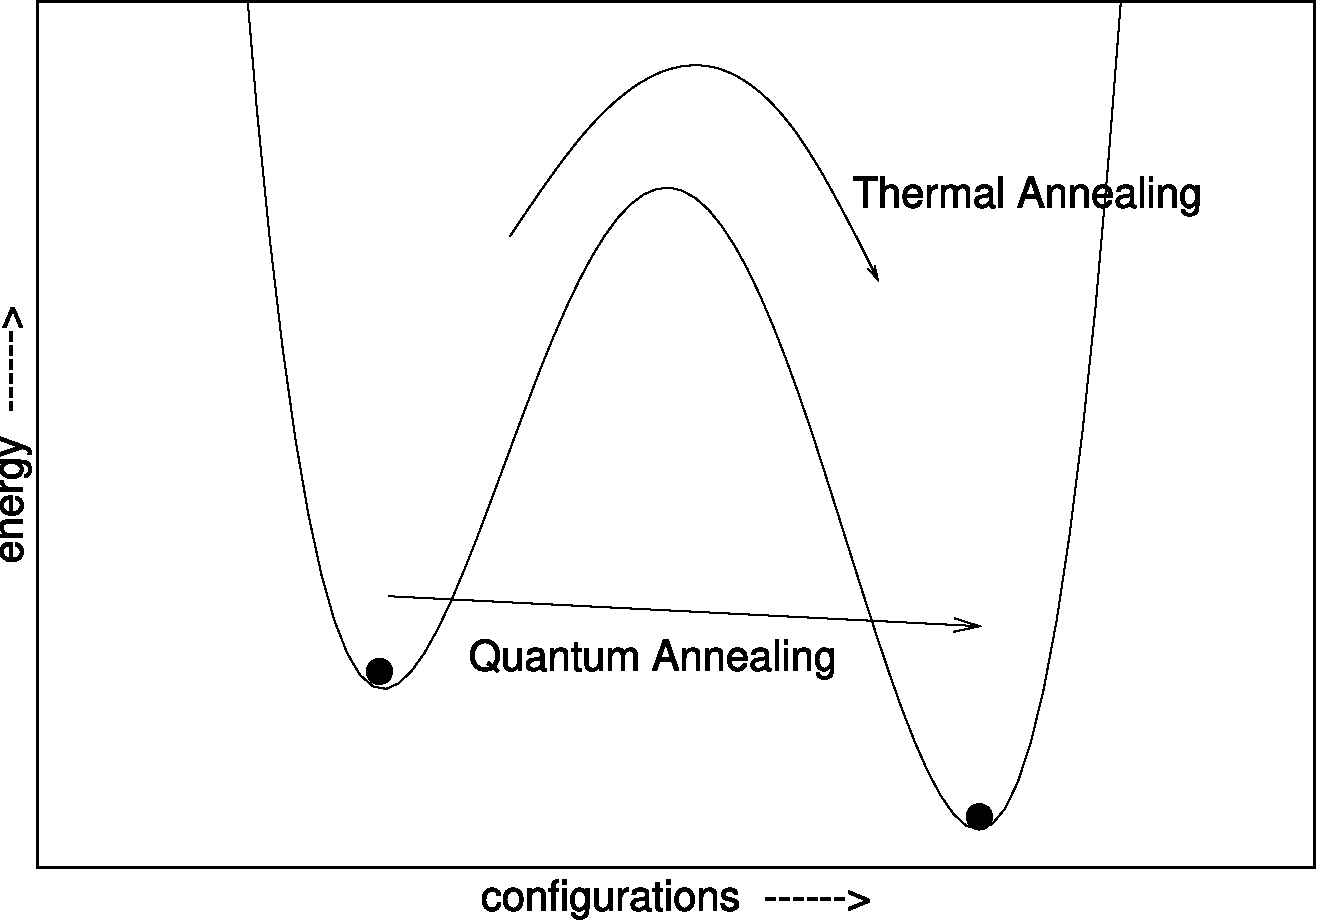
\includegraphics[width=0.9\linewidth]{Graphics/quantum_computing/QA}
	\caption{Simulated annealing e quantum annealing \cite{k2005transverse}}
	\label{fig:qa}
\end{figure}

L'Hamiltoniano disordinante $\mathbf{H}_d$ introduce energia cinetica nel processo di annealing sotto forma di fluttuazioni quantistiche dello spazio delle soluzioni. Diminuire $\Gamma(t)$ avvicina il sistema a $\mathbf{H}_f$ smorzando le fluttuazioni quantistiche. La Figura~\ref{fig:qa} mostra graficamente il vantaggio del QA rispetto alla controparte classica: valori elevati di $\Gamma(t)$ consentono al calcolo di sfuggire ai minimi locali attraverso il \emph{tunneling} attraverso le colline invece di scalarle gradualmente. Ciò consente all'algoritmo di muoversi più velocemente e più lontano nello spazio delle soluzioni nelle fasi iniziali del processo.

Un altro vantaggio del QA è che, durante l'evoluzione, il sistema non si trova in un singolo stato, ma in una sovrapposizione di stati la cui probabilità è definita da $\mathbf{H}(t)$. Questa idea viene adottata anche dagli algoritmi che implementano il QA su architetture classiche. In\marginpar{Simulated quantum\\annealing} questo caso si parla di \emph{simulated quantum annealing} e l'obiettivo è cercare di catturare la proprietà di sovrapposizione rappresentando molti stati in parallelo\footnote{Una discussione più approfondita sul simulated quantum annealing va oltre lo scopo di questo lavoro, ma può essere trovata in \cite{suzuki2005simulated}.}.

\subsubsection*{Formulazione di un problema per l'annealing}
\label{sec:annealing_form}
Vediamo come formulare un problema in modo che possa essere risolto con un \emph{quantum annealer} (una macchina capace di implementare il QA). Otterremo due formulazioni equivalenti che descrivono problemi risolvibili con quantum annealing, simulated annealing o simulated quantum annealing. Per ora ci concentriamo sulla descrizione teorica della formulazione. Per un'implementazione pratica compatibile con un'architettura QA, si veda la Sezione~\ref{sec:ocean}.

\paragraph{Modello di Ising:} è un modello matematico che descrive le transizioni di fase e altre proprietà di un sistema fisico che evolve nel tempo. Il problema è definito da $n$ particelle disposte su un grafo $G = (V, E)$ che può essere descritto come una griglia $d$-dimensionale. Ogni particella può trovarsi in uno stato di spin $\in \Set{+1, -1}$. Chiamiamo \emph{configurazione di spin} $s = s_1,\dots, s_n$ un'assegnazione di spin alle particelle.

Due\marginpar{Forze sulle\\particelle} tipi di forze possono agire sul sistema descritto:
\begin{itemize}
	\item \emph{forze esterne} $h_i$ applicate alle singole particelle;
	\item \emph{forze di interazione} $J_{ij}$ tra vicini nella griglia (due vertici $v_i$ e $v_j$ collegati da un arco $e_{ij}$). Se non ci sono archi tra $v_i$ e $v_j$ assumiamo $J_{ij} = 0$.
\end{itemize}

L'energia di una data configurazione è definita da
\begin{equation}
	\mathbf{H}(s) =  \sum_{i}h_i\cdot s_i + \sum_{j < i} J_{ij}\cdot s_i s_j \ .
	\label{eqn:ising}
\end{equation}

Vediamo come codificare questa funzione energia in un quantum annealer. Considerando una collezione di $n$ qubit $Q = q_1,\dots, q_n$ disposti nella griglia definita dal grafo $G = (V, E)$, lo stato di $Q$ è $\Ket{\Phi} = \Ket{\phi_1, \dots, \phi_n}$. Possiamo tradurre questa energia nell'Hamiltoniano del problema $H_f$:
\begin{equation}
	\mathbf{H}_f =  \sum_{i\in V}h_i\cdot Z\,q_i + \sum_{(i,j) \in E} J_{ij}\cdot Z\,q_i\ Z\,q_j.
\end{equation}
Dove $Z\,q_i$ indica l'applicazione della porta di Pauli $Z$ al qubit $i$. Questo è un Hamiltoniano valido per un algoritmo QA e un quantum annealer è in grado di trovare la soluzione di energia minima.

\paragraph{Problema QUBO:} Il modello di Ising è definito su spin $s_1 \in \Set{+1. -1}$. Una formulazione equivalente, ma più vicina a quella usuale in informatica, è il problema di \emph{Ottimizzazione Binaria Quadratica Non Vincolata} (forma QUBO). In questa formulazione consideriamo $n$ variabili booleane $x_i \in \Set{0,1}$ e, considerando una matrice triangolare superiore $Q_{ij}$ di pesi di dimensione $n\times n$, vogliamo minimizzare la funzione
\begin{equation}
	f_{QUBO}(x) =  \sum_{i, j}Q_{ij}\cdot x_ix_j\ .
	\label{eqn:qubo}
\end{equation}

È \marginpar{Dalla forma QUBO\\alla forma Ising\\e viceversa}possibile dimostrare che un problema in forma QUBO ha sempre una versione corrispondente nella forma del modello di Ising, e per passare da una formulazione all'altra si impone $s_i = 1 - 2 x_i$ \cite{bian2010ising}. È anche possibile dimostrare che lo stato fondamentale del problema in forma QUBO è lo stesso di quello in forma Ising a meno di un offset finito $\delta_e$
\begin{equation}
	\min_{s\in\Set{-1, +1}}  \sum_{i}h_i\cdot s_i + \sum_{j < i} J_{ij}\cdot s_i s_j = \min_{x\in\Set{0, 1}} \sum_{i, j}Q_{ij}\cdot x_ix_j + \delta_e\ .
	\label{eqn:ising_qubo}
\end{equation}

\section{Conclusione}
In questo lavoro abbiamo giustificato l'interesse per il calcolo quantistico mostrando come questo nuovo paradigma si posizioni all'interno dello studio della complessità computazionale e nella definizione delle classi di problemi computazionali.

Abbiamo iniziato definendo i modelli teorici che descrivono la computazione classica, come la macchina di Turing e il modello a circuiti. Partendo da questi, abbiamo classificato i problemi computazionali in base alle risorse necessarie per risolverli.

Abbiamo quindi introdotto teoricamente il calcolo quantistico (attraverso i circuiti quantistici) e mostrato come le classi di problemi computazionali cambiano quando si considera questo nuovo paradigma. In particolare, abbiamo osservato che dimostrare i vantaggi computazionali del paradigma quantistico porterebbe a risultati significativi anche nella computazione classica, rendendo possibile dimostrare che $\textbf{P} \neq \textbf{PSPACE}$.

Il capitolo prosegue poi definendo il paradigma di calcolo quantistico basato su porte, questa volta in modo meno teorico, osservando come un qubit è definito in un modello computazionale e cosa significa applicare una porta quantistica a un sistema di qubit per modificarne lo stato. La sezione sulle porte quantistiche si conclude con l'algoritmo di Deutsch, che mostra una prima accelerazione (anche se solo polinomiale) dei computer quantistici rispetto alle architetture classiche.

Abbiamo concluso il capitolo esaminando un altro approccio al calcolo quantistico, questa volta un approccio analogico: il CAQ. Abbiamo descritto in cosa consiste un algoritmo CAQ e quali condizioni devono essere soddisfatte affinché questo algoritmo ci permetta di ottenere la soluzione al nostro problema. Infine, siamo passati dal modello CAQ universale agli algoritmi QA, perdendo generalità ma rilassando i vincoli imposti alla computazione. Abbiamo derivato due forme per formulare un problema adatto al QA (forma QUBO e forma Ising) e ne abbiamo evidenziato l'equivalenza.

Queste due formulazioni che abbiamo ottenuto sono precisamente l'obiettivo del resto del nostro lavoro: trasformare la conoscenza strutturata, e una query su questa conoscenza, in una formulazione adatta al QA.